
%(BEGIN_QUESTION)
% Copyright 2007, Tony R. Kuphaldt, released under the Creative Commons Attribution License (v 1.0)
% This means you may do almost anything with this work of mine, so long as you give me proper credit

In 1976, an engineer named Bob Metcalfe designed a new type of digital communication standard he dubbed {\it Ethernet}.  A sketch he drew of his new system looked like this:

$$\includegraphics[width=15.5cm]{i02201x01.eps}$$

Explain the basic concept behind Metcalfe's Ethernet system, and why he chose the word ``ether'' to name it.  Also, identify the bit rate (speed) at which his original Ethernet communicated at.

\vskip 20pt \vbox{\hrule \hbox{\strut \vrule{} {\bf Suggestions for Socratic discussion} \vrule} \hrule}

\begin{itemize}
\item{} Identify some disadvantages of the original coaxial-based Ethernet versus modern twisted-pair (with hubs) Ethernet networks.
\end{itemize}

\underbar{file i02201}
%(END_QUESTION)





%(BEGIN_ANSWER)

The basic idea of Ethernet is that there is an electrically passive medium (a coaxial cable) serving as a conduit for signals transmitted by any station connected to that medium.  The transparency and passivity of the network cabling was supposed to be analogous to the ``luminiferous ether'' that was once thought of as filling all space, serving as a medium for electromagnetic waves to exist.

\vskip 10pt

The data rate for the original Ethernet specification was 2.94 Mbps (2.94 million bits per second).

\vskip 10pt

It should be noted that Metcalfe's original Ethernet was an example of a {\it multipoint}, broadcast network.  All stations are allowed to initiate communication, and that communication gets broadcast to all stations connected to that line.  Now, with switching hubs, the ``broadcast'' portion of the description is a bit more limited, but it is still a true multipoint network.

%(END_ANSWER)





%(BEGIN_NOTES)


%INDEX% Networking, Ethernet: Metcalfe's original design

%(END_NOTES)


